\documentclass[11pt]{article}  
%%Read the manual for other options. 

\pagestyle{empty} %%Eliminates page numbers
%%\input rmb_macros
%%Collect your favorite macros in a 
%%separate file

%\input amssym.def
%\input amssym
%\input mssymb
%%Defines additional symbols



\usepackage{graphics}
\usepackage{amsmath,amssymb,amsthm, multicol}
\usepackage[pdftex]{graphicx}
\usepackage[backend=bibtex, sorting=none]{biblatex}
\usepackage{epsf}
%%Use to include pictures. 

%\newcommand{\comment}[1]{}
%\newcommand{\sobolev}[2]{W^{#1,#2}}
%\newcommand{\sobolev}[2]{L^#2_#1}
%%Some examples of macros or new commands.

\addtolength{\oddsidemargin}{-.75in}
\addtolength{\evensidemargin}{-.75in}
\addtolength{\textwidth}{1.5in}
\addtolength{\topmargin}{-1in}
\addtolength{\textheight}{2.25in}
\addbibresource{handout_refs.bib}
%\bibliography{handout_refs}
%%Set margins, defaults are ok. 

\newcommand{\integers}{\mathbb{Z}}


%\bibliography{handout_refs}

\begin{document}
\begin{center}
{\bf \Large Braid Group Cryptography - Liam Hardiman}
\vspace{0.2cm}
\hrule
\end{center}

%\subsection*{Background}
%Let $G$ be a finitely presented group with \textbf{generators} $x_1, x_2, \ldots, x_n$ and \textbf{relators} $r_1 = e$, $r_2 = e$, \ldots, $r_m = e$. For each generator $x_i$ there is a corresponding inverse $x_i^{-1}$. A \textbf{word} in $G$ is a finite string made of the symbols $x_i$ and $x_i^{-1}$. The empty string $e$ is a word that will serve as the identity element. Each relator $r_i$ is a word. 
% A \textbf{finitely presented group} is specified by the following data.
% \begin{enumerate}
% 	\item \textbf{Generators} $x_1, x_2, \ldots, x_n$. Just a set of symbols.
% 	\item \textbf{Relators} $r_1 = e$, $r_2 = e$, \ldots, $r_m = e$. More on these in a moment.
% \end{enumerate}

% \indent For each generator $x_i$ there is a corresponding inverse, $x_i^{-1}$. A \textbf{word} is just a finite string made of the symbols $x_i$ and $x_i^{-1}$. The empty string $e$ is a word and will be the identity element in $G$. The relators are words.\\
% \indent $G$ consists of all \textit{equivalence classes} of words, where two words $u$ and $v$ are equivalent if $u$ can be transformed into $v$ by a finite sequence of cancellations or eliminating/introducing relators.\\
% \indent Equivalently, $G$ is a quotient of the free group on the generators modulo the normal closure of the relators. 

\subsection*{The Word Problem}
The \textbf{word problem} is the decision problem that asks whether two words $u$ and $v$ in a finitely presented group, $G$, are equivalent. In some finitely presented groups this is \textbf{undecidable} -- it is provably impossible to give an algorithm that always outputs a correct answer \cite{nov55}.

\subsection*{The Conjugacy Problem}
The \textbf{conjugacy search problem} asks, given two conjugate words $u$ and $v$ in $G$, find a word $w$ such that $u = w^{-1}vw = v^w$. Like the word problem, this is undecidable in some finitely presented groups.

\subsection*{The Braid Group}
Symbolically, the braid group on $n$ strands has the following presentation
\[
B_n = \langle \sigma_1, \sigma_2, \ldots, \sigma_{n-1}\ |\  \sigma_i\sigma_j\sigma_i = \sigma_j\sigma_i\sigma_j\text{ if }|i-j| = 1,\ \sigma_i\sigma_j = \sigma_j\sigma_i\text{ if }|i-j|>1\rangle.
\]
Visually, imagine two sets of $n$ items arranged in vertical lines on either side of the page. Attach one end of a string to each item on the left side of the page. To each item on the right side attach the other end of one string. This connection is a \textbf{braid}. The strings might cross over or under one another any number of times and we say each such configuration gives a \textit{different} braid.\\
\indent The generator $\sigma_i$ represents the braid formed by crossing strand $i$ under strand $i+1$ and leaving the other strings fixed.
\begin{figure}[h]
\centering
	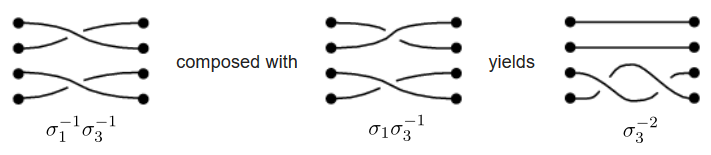
\includegraphics[scale=.61]{composition.PNG}
\caption{Composing two braids in $B_4$}
\end{figure}

\indent Two connections that can be made to look the same by tightening the strings are considered the \textit{same} braid. Composing two braids consists of drawing them next to one another, gluing the points in the middle, and connecting the strands.\\


\noindent \textbf{Theorem (Canonical Form for Braids \cite{ko2000}) : }Every braid, $w$, in $B_n$ has a unique representation called the left-canonical form,
\[
w = \Delta^uA_1A_2\cdots A_p,\quad \text{for some }u\in \integers
\]
where $\Delta$ is a particular braid, the fundamental braid, and the $A_i$'s are braids of a particular form that come from a \textit{finite} subset of $B_n$. Moreover, if $w$ is given as a word of length $\ell$ in the generators $\sigma_1, \sigma_2, \ldots, \sigma_{n-1}$, then this canonical form is computable in time $O(\ell^2n\log n)$. In particular, the word problem is easy in $B_n$.

\subsection*{Diffie-Hellman with Braids \cite{aag99}}
\begin{enumerate}
	\item Alice and Bob publicly agree on subgroups of $B_n$,  $A = \langle a_1, \ldots, a_k\rangle$ and $B = \langle b_1, \ldots b_m\rangle$.
	\item Alice picks a secret word $x$ in $a_1, \ldots, a_k$, $x = x(a_1, \ldots, a_k)$. Bob picks a secret word $y$ in $b_1, \ldots, b_m$, $y = y(b_1, \ldots, b_m)$.
	\item Alice sends $b_1^x, \ldots, b_m^x$ to Bob and Bob sends $a_1^y, \ldots, a_k^y$ to Alice.
	\item Alice computes $x(a_1^y, \ldots, a_k^y) = x^y = y^{-1}xy$. Bob computes $y(b_1^x, \ldots, b_m^x) = y^x = x^{-1}yx$.
	\item Alice multiplies on the left by $x^{-1}$, obtaining $x^{-1}y^{-1}xy$. Bob multiplies on the left by $y^{-1}$ and inverts, obtaining $(y^{-1}x^{-1}yx)^{-1} = x^{-1}y^{-1}xy$. The shared secret is the commutator $[x,y] = x^{-1}y^{-1}xy$.
\end{enumerate}

\subsection*{Security \cite{su06}}
An eavesdropper knows $a_1, \ldots, a_k, b_1, \ldots, b_m$ and $a_1^y, \ldots, a_k^y, b_1^x, \ldots, b_m^x$. It might appear that if they can solve the simultaneous conjugacy search problem (search SCP) then they can obtain the shared secret. But that might not be enough.
\begin{itemize}
	\item If $a_i^{y'} = a_i^y$ for all $i$, it need not be the case that $y' = y$, just that $y' = c_ay$ for some $c_a$ in the centralizer of $A$. Similarly, solving the simultaneous conjugacy problem in the $b_j^x$'s gives $x' = c_bx$ for some $c_b$ centralizing $B$.
	\item The commutator of $x'$ and $y'$ is
	\[
	[x',y'] = (x')^{-1}(y')^{-1}x'y' = x^{-1}c_b^{-1}y^{-1}c_a^{-1}c_bxc_ay,
	\]
	which need not equal $[x,y]$.
	\item However, if $x'$ is in $A$ and $y'$ is in $B$, then $c_b = x'x^{-1}$ and $c_a = y'y^{-1}$ implies that $c_b \in A$ and $c_a\in B$. Consequently, $c_b$ commutes with $y$ and $c_a$, and $c_a$ commutes with $x$ and $c_b$, so we have the equality $[x',y'] = [x,y]$.
\end{itemize}
So evidently, the eavesdropper needs to not only solve the search SCP, but they need these conjugating elements to be words in $A$ and $B$. This combination of problems is called the simultaneous conjugacy separation search problem (SCSSP). 

\subsection*{How Hard Is This to Crack?}
It is currently unknown whether computing the centralizers of $A$ and $B$ reduces to the search SCP. In either case, as of 2014 \cite{ktv14}, there is no known efficient algorithm for computing centralizers of arbitrary subsets of braid groups . Kotov et al.\ \cite{kmmpu18}\ describe an attack on the SCSSP that works experimentally but they don't appear to provide a bound on the complexity.

\printbibliography

\end{document}